\documentclass[12]{article}
\usepackage{hyperref}
\usepackage{graphicx}
\usepackage{listings}
\usepackage{color}
\usepackage{xcolor}
\usepackage[margin=1.0in]{geometry}
\definecolor{dkgreen}{rgb}{0,0.6,0}
\definecolor{gray}{rgb}{0.5,0.5,0.5}
\definecolor{mauve}{rgb}{0.58,0,0.82}

\lstdefinestyle{C++}
{
  frame=tb,
  language=C++,
  aboveskip=3mm,
  belowskip=3mm,
  showstringspaces=false,
  columns=flexible,
  basicstyle={\small\ttfamily},
  numbers=none,
  numberstyle=\tiny\color{gray},
  keywordstyle=\color{blue},
  commentstyle=\color{dkgreen},
  stringstyle=\color{mauve},
  breaklines=true,
  breakatwhitespace=true,
  tabsize=3
}

\lstdefinestyle{bash}
{
    frame=tb,
    language=bash,
    breaklines=true,
    breakatwhitespace=true,
    tabsize=3,
    backgroundcolor=\color{white},
    basicstyle=\scriptsize\color{black}\ttfamily
}

\title{ACSL TurtleBot3 e-Manual}

\date{June 2020}
\renewcommand\thesection{\arabic{section}}
\renewcommand\thesubsection{\thesection.\arabic{subsection}}

\begin{document}

\makeatletter
    \begin{titlepage}
        \begin{center}
            
\includegraphics[width=0.7\linewidth]{images/ACSL_Logo.jpg}\\[4ex]
            {\huge \bfseries  \@title }\\[52ex]  
            {\large \@date}
        \end{center}
    \end{titlepage}
\makeatother

\tableofcontents
\newpage

\section*{Abstract}
   
This guide documents the changes made to TurtleBot3 software to meet the requirements of ACSL research group. It contains instructions on setting up the robot and code documentation.
       
\addcontentsline{toc}{section}{Abstract}
\newpage

\section{Overview and Setup}

TurtleBot3 is a small ROS-based mobile robot. The TurtleBot3 can be customized by changing the source code and addition of new hardware. TurtleBot3 Waffle Pi is equipped with a Raspberry Pi Camera Module (v2), a 360-degree Laser Distance Sensor (LDS) and Dynamixel XM430 210-T motors.

TurtleBot3 architecture is described in the following image.\\

\begin{center}
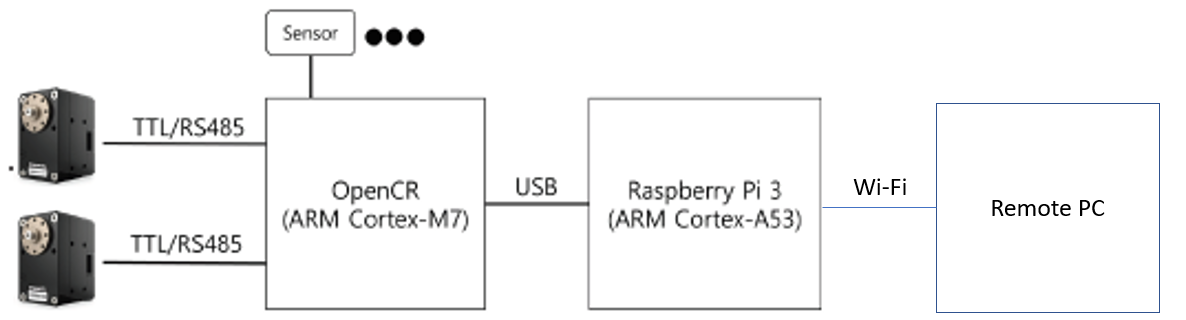
\includegraphics[width=0.7\linewidth]{images/tb3_architecture.png}\\
\end{center}

The four major components of TurtleBot3 are 
\begin{enumerate}
	\item {Raspberry Pi 3B+ Single Board Computer (SBC).}
	\item {OpenCR Embedded System Board.}
	\item {LDS and Camera Sensors.}
	\item {Dynamixel Actuators.}
\end{enumerate}

Raspberry Pi has a WiFi module built onto the board which connects to a computer, known as the Remote PC. Remote PC is used to send commands for SLAM and Navigation to TB3 and visualization of the sensor data is also performed on the remote PC.

There is a one time setup that needs to be performed on the Remote PC, Raspberry Pi and OpenCR board. Most of the software is located in the form of a binary file that is burnt to the EEPROM of the STM32F746 chip on the OpenCR board. As the software used for ACSL projects is custom, it is burnt using Arduino IDE.
 
\subsection{Remote PC Setup}

To begin you will need to install the appropriate ROS version on your remote PC. The remote PC will be running ROS Melodic (EOL date: May 2023). 
The single board computer on Turtlebot3 will be running ROS Kinetic (EOL date: April 2021) for the ease of setup since ROS Melodic requires manual compilation when using Rasbian. 
No problem has yet been found by us on the communication between these 2 releases. 

The following page from ros.org describes the process for adding and installing all necessary packages to your ROS Environment.

\url{http://wiki.ros.org/melodic/Installation/Ubuntu} 

Note that please do not follow the Turtlebot3 guide to configure the ROS environment on the remote PC \textbf{(Step 6.1.1-6.1.3)}. 
Instead, simply follow the instructions in the link above.

Then, install required dependencies
\begin{lstlisting}[style=bash]
sudo apt install ros-melodic-joy ros-melodic-teleop-twist-joy ros-melodic-teleop-twist-keyboard ros-melodic-laser-proc ros-melodic-rgbd-launch ros-melodic-depthimage-to-laserscan ros-melodic-rosserial-arduino ros-melodic-rosserial-python ros-melodic-rosserial-server ros-melodic-rosserial-client ros-melodic-rosserial-msgs ros-melodic-amcl ros-melodic-map-server ros-melodic-move-base ros-melodic-urdf ros-melodic-xacro ros-melodic-compressed-image-transport ros-melodic-rqt-image-view ros-melodic-gmapping ros-melodic-navigation ros-melodic-interactive-markers
\end{lstlisting}

\textbf{Warning! We have used other dependencies but we didn't keep documentation, we need to figure out all the deps that we have used.}

The next step is to configure network settings for permanent use. 
The Remote PC will be controlling the turtlebot pc via wifi using SSH protocol. 
Steps for configuring the wifi on the remote pc can be found here.

\url {https://emanual.robotis.com/docs/en/platform/turtlebot3/pc_setup/#network-configuration} \\

For this project we will use the Linksys Router on the \textbf{Linksys04294} network. It is helpful to write down the IP address of the remote pc, since you will need it later to setup the turtlebot pc network settings.\\\\

Then, clone and build the git repository. 
\begin{lstlisting}[style=bash]
git clone https://github.com/hanyiabc/ASCL_turtlebot3.git
cd ASCL_turtlebot3/
catkin_make
\end{lstlisting}

Add this environment variable to .bashrc and refresh the environment variables
\begin{lstlisting}[style=bash]
echo "export TURTLEBOT3_MODEL=waffle_pi_effort_controller" >> ~/.bashrc
source ~/.bashrc
\end{lstlisting}
On the original Turtlebot code, this environment variable is used to define the model of the Turtlebot, possible values are \textbf{waffle, waffle\_pi, burger}. 
Difference URDF file is loaded based on this environment variable. 
For this project however, we defined new URDF files for effort control, so we need to set the environment variable to what we have defined as the name of the model for effort control. 
\subsection{Rasberry Pi SBC Setup}

Now it is time to look at the turtlebot SBC. For the turtlebot 3 Waffle Pi model, the on board PC is a raspberry PI. 
This step requires a micro SD card with adapter, a monitor with an HDMI input, a USB keyboard and mouse, and a power source for the turtlebot. 
ROBOTIS provides a prebuilt desktop environment for the turtlebot with ROS kinetic. Instructions for flashing this distribution can be found here (\textbf{Step 6.2.1.2 Install Linux Based on Raspbian, Do not use the other two methods.}).\\
\url {https://emanual.robotis.com/docs/en/platform/turtlebot3/raspberry_pi_3_setup/#raspberry-pi-3-setup}

To use the Raspberry PI without a physical access, use SSH. Example SSH command:

\begin{lstlisting}[style=bash]
ssh pi@YOUR_RASPBERRY_PI_IP
\end{lstlisting}

For the ease of use, VNC configuration is recommended. This provide remote desktop funtionality. In case of Debian Stretch (the version that the manual will use), install Real VNC by running this command on the Raspberry PI:
\begin{lstlisting}[style=bash]
sudo apt update
sudo apt install realvnc-vnc-server realvnc-vnc-viewer
\end{lstlisting}
THen enable VNC server by 
\begin{lstlisting}[style=bash]
sudo raspi-config
\end{lstlisting}
Then navigate to Interfacing Options.
Scroll down and select VNC - Yes.


Ubuntu Desktop 18.04 comes with VNC client Remmina.
On Windows, use VNC viewer
\url{https://www.realvnc.com/en/connect/download/viewer/}
\subsection{OpenCR Setup}

The original source code for TurtleBot3 used the inbuilt PID controller of the Dynamixel XM430 210-T actuators. However, to benchmark the performance of the controllers, the control is shifted from the motors to higher level software such as Simulink or a custom ROS node.

The source code for OpenCR can be downloaded by cloning the following repository.

\url {https://github.com/hanyiabc/ASCL_turtlebot3.git}

Arduino IDE can be used to burn the \textbf{turtlebot3\_core.ino} file located in \textbf{ACSL\_turtlebot3/src/turtlebot3\_core} directory. Instructions for setting up the Arduino IDE for TurtleBot3 can be found in the following link.

\url {https://emanual.robotis.com/docs/en/parts/controller/opencr10/#arduino-ide}

\newpage
\section{Repository Introduction}
The repository is a catkin workspace. A catkin workspace has a src folder that contains multiple packages. The worth-mentio ning ones are:
\begin{itemize}
	\item[--] hls\_lfcd\_lds\_driver
    \item[--] raspicam\_node
    \item[--] ros\_control
    \item[--] simulink
    \item[--] turtlebot3
    \begin{itemize}
        \item[--] turtlebot3\_bringup
        \item[--] turtlebot3\_navigation
        \item[--] turtlebot3\_slam
        \item[--] turtlebot3\_teleop
    \end {itemize}
    \item[--] turtlebot3\_core
    \item[--] turtlebot3\_setup\_motor
    \item[--] turtlebot3\_simulations
\end{itemize} 

Not all packages are catkin package. \textbf{simulink}, \textbf{turtlebot3\_core} \textbf{turtlebot3\_setup\_motor} are all just directories. 
All the rests are properly configured as catkin packages, meaning all the nodes defined under the package will be compiled when running the \textbf{catkain\_make} command. 

\textbf{hls\_lfcd\_lds\_driver} and \textbf{raspicam\_node} are drivers for the PI Camera and lidar. 
These will be running in the single board computer. 

\textbf{ros\_control} contains all the configuration and nodes necessary to control the robot. 
It contains the PID controller configurationl, PID gains, etc.
Two launch files are included for controlling the robot in either the simulations or in the physical world. They are:

\begin{itemize}
	\item[--] turtlebot3\_control.launch
	\item[--] turtlebot3\_control\_simulation.launch
\end{itemize}  
These launch file are not ran directly, instead they are inlcuded by other launch file that we will introduce later.
The PID gains can be tuned by either changing the parameters in the launch file or use a ros package called rqt\_reconfiture to adjust parameters with sliders at runtime. 
There are 2 nodes under the \textbf{ros\_control} package. They are \textbf{differential\_driver.py} and \textbf{ros\_control\_node}. 
The \textbf{differential\_driver.py} is a Python ros node that split the incoming \textbf{\//cmd\_vel} messages into left and right velocity for the differential drive robot based on vehicle geometry. 
The \textbf{\/cmd\_vel} is the standard topic that ROS nav stack used to output the velocity command. It commands the robot in terms of translational velocity and orientation. 
The \textbf{ros\_control\_node} is a C++ ros node compiled from the soruce file: \textbf{message\_redirect.cpp}. 
This node simply takes the left and right wheel angular velocities feedbacks from \/joint\_states converts them to linear velocities and publish them into 2 Float64 messages for the PID controller to read.


The directory \textbf{simulink} contains all the MATLAB scrips and Simulink models for controlling the robot with MATLAB 

\textbf{turtlebot3\_bringup} contains all the launch file for bringing up the Turtlebot in the SBC and the remote PC. 
\textbf{turtlebot3\_physical\_nav\_control.launch} was added to the bringup package to provide a convinient one-file launch that will handles everything. 
This launch file brings up the turtlebot on the remote PC, runs the velocity control and the navigation stack with SLAM. A simulation version will be provided in the future.

\textbf{turtlebot3\_description} contains the URDF and Gazebo descripion of the turtlebot for both simulation and physical robot. 

For Waffle Pi, \textbf{turtlebot3\_waffle\_pi.gazebo.xacro}
and \textbf{turtlebot3\_waffle\_pi.urdf.xacro}
are provided by the turtlebot package, however, for effort control, we added 2 more files. 
They are: \textbf{turtlebot3\_waffle\_pi\_effort\_controller.gazebo.xacro}
and \textbf{turtlebot3\_waffle\_pi\_effort\_controller.urdf.xacro}
These files are derived from the original descriptions and added ability to control effort in both the simulation and the physical robot. 

\textbf{turtlebot3\_navigation} contains the default configuration for running the ROS navigation stack with the Turtlebot.
A new launch file \textbf{turtlebot3\_navigation\_no\_map.launch} was created. This launch file derived from the original navigation launch file, but the difference is that this configuration doesn't need a SLAM map for localizatin. 
The localizatin is provide by SLAM instaed of Adaptive Monte Carlo Localizatin. The default launch file \textbf{turtlebot3\_navigation.launch} will run navigation assuming that a SLAM map has been drawn by running SLAM before. In this configuration, 
localizatin is provided by AMCL. 


\section{Torque Control using Dynamixel}
       
Dynamixel is a microcontroller based actuator with in-built PID controller. OpenCR communicates with Dynamixel using packet communication via TTL/RS45 ports. 

Hardware level abstraction is achieved via Dynamixel SDK library available in several programming languages. (CPP used in our case.)
Dynamixel register addresses and byte sizes for both RAM and EEPROM memory provided in control table. RAM is most frequently used memory for robot applications, while startup settings are stored on EEPROM.

The Control Table is a structure that consists of multiple Data fields to store status or to control the device. Users can check current status of the device by reading a specific Data from the Control Table with Read Instruction Packets. WRITE Instruction Packets enable users to control the device by changing specific Data in the Control Table. Packet sizes range from 1 – 4 bytes.

Following is a snapshot of the Dynamixel EEPROM Control Table. Each data in the Control Table is restored to initial values when the device is turned on. Default values in the EEPROM area (addresses 0-63) are initial values of the device (factory default settings). If any values in the EEPROM area are modified by a user, modified values will be restored as initial values when the device is turned on. Initial Values in the RAM area are restored when the device is turned on.

\begin{center}
	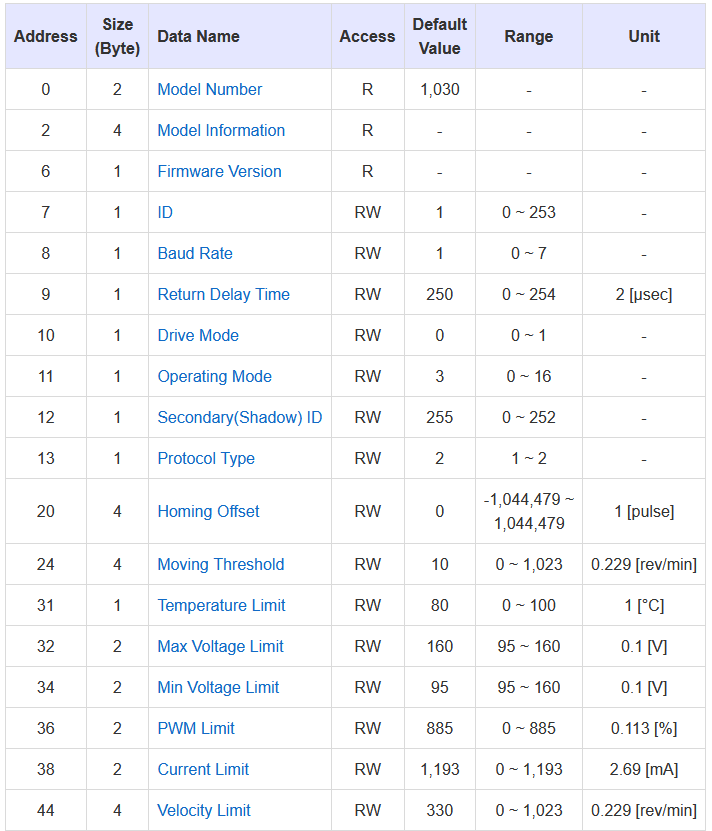
\includegraphics[width=0.7\linewidth]{images/dxl_eeprom.png}\\
\end{center}

For the purpose of torque control, the operating mode of the dynamixel motor needs to be set to \textbf{MODE 0}. This can be done using the motor setup code in the git repository.
To change the operating mode to \textbf{MODE 0}, flash the turtlebot3\_setup\_motor firmware to the OpenCR board while the motors are connected to the board. 
Open up a serial terminal with Arduino or Terraterm, under the serial termianl, you will see the following options:
\begin{lstlisting}[style=bash]
    1. setup left  motor
    2. setup right motor
    3. test  left  motor
    4. test  right motor
    5. setup left  motor for current control
    6. setup right  motor for current control
    7. test left  motor for current control
    8. test right  motor for current control
>> 
\end{lstlisting}
The first 4 options comes with the OpenCR Arduino library. The last 4 options are added based on the first 4 options and they configure the left and right motors for torque control.
For now, the current is limited to half of the highest value to avoid damage to the hardware. If changes are needed, the source code needs to be modified and the motors has to be setup again. 
To setup the left motor, simply put 5 in the termianl and press enter. Wait until it says it's finished. Then use option 6 for the right motor.
After the setup is done, use option 7 and 8 to test the motor. The test option apply a small torque to the motor for one second and stops for one second. Make sure both motors are tested then, flash the turtlebot3\_core firmware back.
Once the operating mode is set. The OpenCR code is changed to write torque values to the Dynamixel RAM addresses, when the robot is live. The addresses that are useful for this purpose are given in the image below.

\begin{center}
	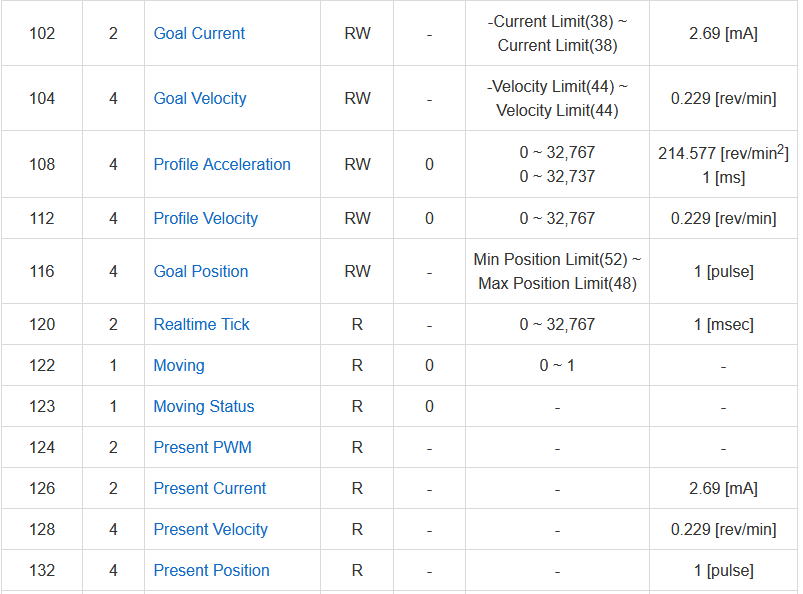
\includegraphics[width=\linewidth]{images/dxl_control_table.png}\\
\end{center}

The code that change the operating mode of the motor is below. 

\lstinputlisting[style=C++, firstline=511, lastline=561]{../src/turtlebot3_setup_motor/turtlebot3_setup_motor.ino}

The code used to test the torque control after setup is below. 
\lstinputlisting[style=C++, firstline=453, lastline=510]{../src/turtlebot3_setup_motor/turtlebot3_setup_motor.ino}

The OpenCR Arduino library comes with a TurtleBot3MotorDriver class that helps controlling the 2 motors by commanding velocities. 
A new class TurtleBot3MotorTorqueDriver was derived (strictly speaking, not inherited, instead just copied and pasted) from the TurtleBot3MotorDriver with new member functions added for controlling the torque instead of velocities. 
The class is defined as below
\lstinputlisting[style=C++, firstline=38, lastline=74]{../src/turtlebot3_core/turtlebot3_motor_torque_driver.h}

The following member functions is added to the TurtleBot3MotorDriver class, which takes in input torque value and converts it into appropriate register values for writing to the appropriate addresses.
\lstinputlisting[style=C++, firstline=275, lastline=291]{../src/turtlebot3_core/turtlebot3_motor_torque_driver.cpp}

\textbf{CURRENT\_TO\_OUTPUT} and \textbf{TORQUE\_TO\_CURRENT} are macro functions that does the conversions from torque to current and current to a 2 byte value that the microcontroller undertand. 
All the necessary macros are defined as
\lstinputlisting[style=C++, firstline=23, lastline=36]{../src/turtlebot3_core/turtlebot3_motor_torque_driver.h}

This conversion is based on a linear approximation of the actuator performance graph.

\begin{center}
	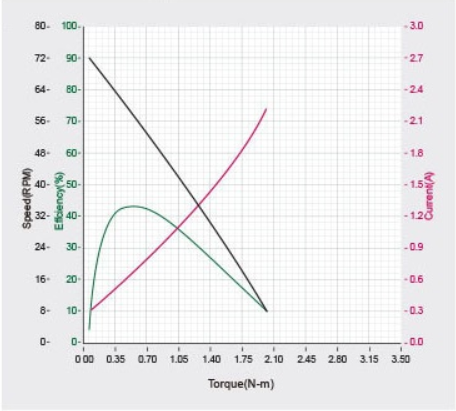
\includegraphics[width=\linewidth]{images/xm430_performance.png}\\
\end{center}

This function below takes the converted value and write to both motors using the Dynamixel SDK APIs. 
\lstinputlisting[style=C++, firstline=227, lastline=249]{../src/turtlebot3_core/turtlebot3_motor_torque_driver.cpp}

Subscribers are added to subscribe to the topics \/left\_torque \/right\_torque. 
The following use the function defined above and write the correspounding values to the correct memory location of the Dynamixel motor controller when new message comes in. 
When there is no new message, it will timeout and write zeros to both motors. 

\lstinputlisting[style=C++, firstline=87, lastline=99]{../src/turtlebot3_core/turtlebot3_core.ino}

The Odometry publisher is in the microcontroller. Since the built-in differential drive plugin which provides Odometry was removed to use our own controller,
An Odometry publisher was added to the system. The source code is below. 

\lstinputlisting[style=C++, firstline=87, lastline=99]{../src/turtlebot3_core/turtlebot3_core.ino}


\newpage

\section{Bring up the Turtlebot}
Once the remote PC and Raspberry PI are setup according to the instructions provieded in the previous sections, 
Follow the instructions below to bring up turtlebot.  \\
On Remote PC
\begin{lstlisting}[style=bash]
    roscore
\end{lstlisting}
On SBC
\begin{lstlisting}[style=bash]
    roslaunch turtlebot3_bringup turtlebot3_robot.launch
\end{lstlisting}

On Remote PC, once you followed the instructions for building the workspace and setting up the environment variables,  
load the environment variables related to this workspace (Note: This has to be done everytime you want to run something from this workspace from a new termianl)
\begin{lstlisting}[style=bash]
cd ASCL_turtlebot3/
source devel/setup.bash
\end{lstlisting}

To run teleop to control the Turtlebot with keyboard.
\begin{lstlisting}[style=bash]
roslaunch turtlebot3_teleop turtlebot3_teleop_key.launch
\end{lstlisting}

To run the navigation with PID velocity effort controller and SLAM (with localizatin provided by SLAM and no initial map required) on the physical robot. 
\begin{lstlisting}[style=bash]
roslaunch turtlebot3_bringup turtlebot3_physical_nav_control.launch 
\end{lstlisting}

To run the navigation with PID velocity effort controller and SLAM (with localizatin provided by SLAM and no initial map required) on Gazebo for simulation.  
\begin{lstlisting}[style=bash]
roslaunch turtlebot3_bringup turtlebot3_sim_nav_control.launch 
\end{lstlisting}

To run SLAM only to draw maps
Choose a pre-defined Gazebo world from the following:

\begin{itemize}
    \item[--] turtlebot3\_empty\_world.launch
    \item[--] turtlebot3\_world.launch
    \item[--] turtlebot3\_house.launch
    \item[--] turtlebot3\_stage\_1.launch
    \item[--] turtlebot3\_stage\_2.launch
    \item[--] turtlebot3\_stage\_3.launch 
    \item[--] turtlebot3\_stage\_4.launch
\end {itemize}
For example, if \textbf{turtlebot3\_world.launch} is chosen, run the following command to bring up a virtual Turtlebot on Gazebo for simulation
\begin{lstlisting}[style=bash]
roslaunch turtlebot3_gazebo turtlebot3_world.launch
\end{lstlisting}
\newpage
Then, run the following commands to launch the SLAM nodes and remote control using keyboard. 
\begin{lstlisting}[style=bash]
roslaunch turtlebot3_slam turtlebot3_slam.launch slam_methods:=gmapping
roslaunch turtlebot3_teleop turtlebot3_teleop_key.launch
\end{lstlisting}
Once you are satisfied with the map, save the map by running
\begin{lstlisting}[style=bash]
rosrun map_server map_saver -f ~/map
\end{lstlisting}
% TODO: Add figure from rqt_graph to illustrate topics and massages and connection between nodes, 
% TODO: add graph from tf view_frams to illustrate the TF tree 

\section{Syncing Time using NTP Server and Client}

Raspberry Pi and Odroid SBCs do not have a hardware clock, and therefore it relies on an active internet connection to fetch the accurate time from Ubuntu time server. However, this is not possible as Linksys router, does not have internet access.\\
Every time SBC boots up, the time has to be updated. The time on the Remote PC and the SBC have to be synced up in order for the various transformations to work for the purpose of running SLAM and Navigation in the ACSL Lab Environment. Hence, to sync up time between these two machines, NTP protocol is being used.\\
NTP or Network Time Protocol is a protocol that is used to synchronize all system clocks in a network to use the same time. When we use the term NTP, we are referring to the protocol itself and also the client and server programs running on the networked computers. NTP belongs to the traditional TCP/IP protocol suite and can easily be classified as one of its oldest parts.\\
When you are initially setting up the clock, it takes six exchanges within 5 to 10 minutes before the clock is set up. Once the clocks in a network are synchronized, the client(s) update their clocks with the server once every 10 minutes. This is usually done through a single exchange of message(transaction). These transactions use port number 123 of your system.\\
In this section, a step-by-step procedure is described on how to:
\begin{itemize}
	\item{Install and configure the NTP server on a Ubuntu machine.}
	\item{Configure the NTP Client to be time synced with the server.}
\end{itemize}
These instructions are taken from \url{https://vitux.com/how-to-install-ntp-server-and-client-on-ubuntu/}. However, it is advised that the following instructions are followed as there are some project specific changes that have been made.
\subsection{Configure NTP Server on the Remote PC} 
Open Terminal and run the following commands \textbf{on the remote PC}
\begin{lstlisting}
    sudo apt-get update
    sudo apt-get install ntp
\end{lstlisting}
Most likely NTP will already be installed on the machine. After installation, the configuration file needs to be altered and server pools closest to the PC location needs to be added. This step is optional, as most likely the servers will be configured correctly.
\begin{lstlisting}
    sudo gedit /etc/ntp.conf
\end{lstlisting}
Replace/edit the server pools with the following.
\begin{lstlisting}
    	pool 0.us.pool.ntp.org iburst
	pool 1.us.pool.ntp.org iburst
	pool 2.us.pool.ntp.org iburst
	pool 3.us.pool.ntp.org iburst
\end{lstlisting}
Save and close the configuration file. In order for the above changes to take effect, you need to restart the NTP server. The time from these servers will be synced with the time on the remote PC. as it has internet access. This will make sure that the NTP server clock is accurate.
\begin{lstlisting}
    sudo service ntp restart
\end{lstlisting}
Run the following command to check if the NTP server is configured properly. You should see the remote PC connecting to various servers.
\begin{lstlisting}
    sudo service ntp status
\end{lstlisting}
Finally, the system’s UFW firewall needs to be configured so that incoming connections can access the NTP server at UDP Port number 123. This is the most important step, as it will configure the remote PC to allow client connections.
\begin{lstlisting}
    sudo ufw allow from any to any port 123 proto udp
\end{lstlisting}
Now the Ubuntu host machine is configured to be used as an NTP server. Please take a note of the IP address of the remote PC \underline{when it is connected to the appropriate router.} IP address of a machine depends on which router it is connected to, and hence is not constant. We will need this address in the next step.
\subsection{Configure NTP Client on the SBC}
The \texttt{ntpdate} command will let you manually check your connection configuration with the NTP-server. Only in this case, the server would be the one that we specify. It should already be installed on the SBC, but in case it is not, run the following command \textbf{on the SBC}.
\begin{lstlisting}
    sudo apt-get install ntpdate
\end{lstlisting}
As the SBC will be a client to the host we set up on the remote PC, we need to modify the hosts file for NTP.
\begin{lstlisting}
    sudo gedit /etc/hosts
\end{lstlisting}
Now add your NTP server’s IP (remote PC IP address noted in the previous step) and specify a hostname. Assuming that the remote PC IP address is \texttt{192.168.1.183} and the server has to be named \texttt{ACSLServer}, add the following line to this file:
\begin{lstlisting}
    192.168.1.183	ACSLServer
\end{lstlisting}
Save and close the NTP hosts file. Because we want our client to sync time with the NTP server, the \texttt{timesyncd} service on the client machine needs to be disabled by running the following command.
\begin{lstlisting}
	sudo timedatectl set-ntp off
\end{lstlisting}
Now, we need to specify this NTP server on the remote PC in the NTP configuration file of the client. If \texttt{NTP} is not installed install it using the following command.
\begin{lstlisting}
	sudo apt-get install ntp
\end{lstlisting}
Now we want our client machine to use our own NTP host server to be used as the default time server. For this, we need to edit the \texttt{/etc/ntp.conf} file on the client machine.
\begin{lstlisting}
	sudo nano /etc/ntp.conf
\end{lstlisting}
Add the following line to the file before the list of other servers. There should be a comment indicating the location where new servers can be added, although this is only for readability and functionality shouldn't be affected.
\begin{lstlisting}
	server ACSLServer prefer iburst
\end{lstlisting}
Finally restart the \texttt{NTP} service and the time should be synced.
\begin{lstlisting}
	sudo service ntp restart
\end{lstlisting}
Now your client and server machines are configured to be time-synced. You can view the time synchronization queue by running the following command:
\begin{lstlisting}
	ntpq -p
\end{lstlisting}
If \texttt{ACSLServer} is seen in the list of servers then the client is properly configured.\\
Finally the timezone needs to be set on the SBC to \texttt{America/New-York}. On the Odroid XU4 running \texttt{Ubuntu} with \texttt{MATE} desktop, it is a simple command line instruction as follows.
\begin{lstlisting}
	sudo timedatectl set-timezone America/New-York
\end{lstlisting}
This command may not work on the Raspberry Pi 3B+, but the timezone can be changed using the \texttt{raspi-config} utility.\\
Once the timezones are set, the SBCs are configured properly.

\end{document}
